\documentclass{beamer}

\usepackage{amsmath} % for mathematical symbols and formatting

\title{Rational Fractal Spline}
\author{Kritika Gahlawat, Neha Rana , Monika , Sapna}
\date{}

\begin{document}



% Slide 1: Introduction
\frame{\titlepage}

\begin{frame}{Introduction to Fractal Interpolation}
    \begin{itemize}
        
 \item Fractal interpolation is a modern technique in approximation theory used to fit and analyze scientific data.
       \item The graph of these FIF can be used to approximate image component such as the profiles of mountains ranges, the tops of clouds and horizons over forests.
        \item This method utilizes an iterated function system (IFS) with rational functions of the form \( \frac{p_i(x)}{q_i(x)} \).
        \item Here, \( p_i(x) \) and \( q_i(x) \) are cubic polynomials that include two shape parameters.
        







    \end{itemize}
\end{frame}

\begin{frame}{Advantages of Rational Cubic Fractal IFS}
    \begin{itemize}
        \item The rational cubic IFS provides additional flexibility over classical rational cubic interpolants.
        \item This flexibility arises from the inclusion of scaling factors and shape parameters.
        \item Classical rational cubic functions are a special case of the proposed fractal interpolants.
        
    \end{itemize}
\end{frame}



\begin{frame}{Shape Preservation}
    \begin{itemize}
        \item The fractal interpolation scheme is computationally efficient and adaptable (local, moderately local, or global) based on scaling factors and shape parameters.
        \item Sufficient conditions on scaling factors and shape parameters ensure that the interpolation function preserves shape:
        \begin{itemize}
            \item Monotonicity
            \item Positivity
            \item Convexity
        \end{itemize}
        
    \end{itemize}
\end{frame}
\begin{frame}{Given Data and IFS}
    \begin{itemize}
        \item Consider a data set \(\{(x_i, f_i), i = 1, 2, \ldots, n\}\), where \( x_1 < x_2 < \cdots < x_n \).
        
    \end{itemize}

    \begin{itemize}
        \item Define the IFS \( I^* = \{ \mathbb{R}^2; w_i(x, f) = (L_i(x), F_i(x, f)), i = 1, 2, \ldots, n - 1\} \).
        \item Where:
        \[
        L_i(x) = a_i x + b_i
        \]
        \item \( L_i(x) \) satisfies the condition \\
        \[L_i(x_1) = x_i, L_i(x_n) = x_i+1.\] 
    \end{itemize}

    \begin{itemize}
        \item \( F_i(x, f) = \alpha_i f + r_i(x) \), where:
        \[
        r_i(x) = \frac{p_i(x)}{q_i(x)}
        \]
        \end{itemize}
        \end{frame}
        \begin{frame}
        \begin{itemize}
        \item \( p_i(x) \) and \( q_i(x) \) are cubic polynomials, and \( q_i(x) \neq 0 \quad \forall x \in [x_1, x_n] \).
        \item \[
p_i(x) \equiv P_i(\theta) = U_i (1 - \theta)^3 + M_i \theta (1 - \theta)^2 + N_i \theta^2 (1 - \theta) + Z_i \theta^3,
\]
\[
q_i(x) \equiv Q_i(\theta) = (1 - \theta)^3 + v_i \theta (1 - \theta)^2 + w_i \theta^2 (1 - \theta) + \theta^3
\]
\item Where \( U_i \), \( M_i \), \( N_i \), and \( Z_i \), for \( i = 1, 2, \dots, n - 1 \), are real parameters  as follows:

\[
U_i = f_i - \alpha_i f_1,
\]
\[
Z_i = f_{i+1} - \alpha_i f_n,
\]
\[
M_i = v_i f_i + h_i d_i - \alpha_i \left[(x_n - x_1) d_1 + f_1 v_i\right],
\]
\[
N_i = w_i f_{i+1} - h_i d_{i+1} + \alpha_i \left[(x_n - x_1) d_n - f_n w_i\right].
\]


        \item \( |\alpha_i| < a_i \), for \( i = 1, 2, \ldots, n - 1 \).
    \end{itemize}
\end{frame}

\begin{frame}{Derivative Conditions}
    \begin{itemize}
        \item Let \( F'_i(x, f) = \frac{\alpha_i f + r'_i(x)}{a_i} \), where \( r'_i(x) \) is the derivative of \( r_i(x) \) with respect to \( x \).
        \item Boundary conditions:
        \[
        F_i(x_1, f_1) = f_i, \quad F_i(x_n, f_n) = f_{i+1}
        \]
        \[
        F'_i(x_1, f_1) = d_i, \quad F'_i(x_n, f_n) = d_{i+1}
        \]
        \item for \( i = 1, 2, \ldots, n - 1 \).
        \item \(h_i=x_{i+1}-x_i\;\;;i=1\;to\; n\)
        \item  \( d_i \) (\(i = 1, 2, \ldots, n\)) be the derivative values at the knots.
    \end{itemize}
    
        \begin{itemize}
        \item The value of ends points is given by:
        \[
        d_1 =
        \begin{cases}
            0, & \text{if } \Delta_1 = 0, \\
            \Delta_1 + \frac{(\Delta_1 - \Delta_2) h_1}{h_1 + h_2}, & \text{otherwise}.
        \end{cases}
        \]
    \end{itemize}
        \begin{itemize}
        \item For \( d_n \):
        \[
       d_n =
        \begin{cases}
            0, & \text{if } \Delta_{n-1} = 0, \\
            \Delta_{n-1} + \frac{(\Delta_{n-1} - \Delta_{n-2}) h_{n-1}}{h_{n-1} + h_{n-2}}, & \text{otherwise}.
        \end{cases}
        \]
    \end{itemize}
    
    
\end{frame}
\begin{frame}{}
    \begin{itemize}
        \item The value of \( d_i \) for \( i = 2, 3, \ldots, n - 1 \) is given by:
        \[
        d_i =
        \begin{cases}
            0, & \text{if } \Delta_{i-1} = 0 \text{ or } \Delta_i = 0, \\
            \frac{\Delta_i h_{i-1} + \Delta_{i-1} h_i}{h_i + h_{i-1}}, & \text{otherwise}.
        \end{cases}
        \]
    \end{itemize}
     \begin{itemize}
        \item The variable \(\theta\) is defined as:
        \[
        \theta = \frac{x - x_1}{x_n - x_1}, \quad x \in [x_1, x_n].
        \]
    \end{itemize}
    \begin{itemize}
        \item Then the attractor of IFS is the graph of rational cubic FIF.

    \end{itemize}
\end{frame}
\begin{frame}{Shape Preservation in Fractal Interpolation}
    \textbf{Problem:} \\
    For an arbitrary selection of scaling factors and shape parameters, the rational cubic fractal interpolation function (FIF) may fail to maintain desired shape properties:
    
    \begin{itemize}
        \item \textbf{Monotonicity}: The curve may oscillate, even if the data is monotonic.
        \item \textbf{Positivity}: The interpolation could dip below zero, even if the data is positive.
        \item \textbf{Convexity (Concavity)}: The curvature may not reflect the original data's convex or concave shape.
    \end{itemize}
    \item This is very similar to the ordinary spline schemes that do not
provide the desired shape features of a data.Thus some
mathematical treatment is required to achieve a monotonicity,
positivity, and convexity (concavity) preserving rational cubic spline
FIF for a given data

    
\end{frame}
\begin{frame}{Approach to solve the problem}

\item There are two approach to address this:
\begin{itemize}
    \item Trail and Error= Manually adjusting the scalling factor and shape parameter but it can work sometime usually not very efficient and precise.
    \item Automated Method= Develop automated process to compute the appropriate scalling factor and shape parameter that preserve desired shape properties 
\end{itemize}

    


    
\end{frame}
\begin{frame}{Figure}

    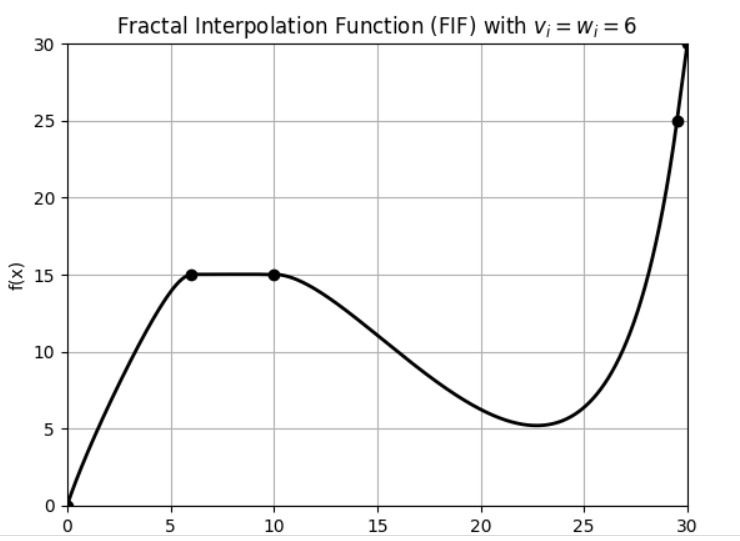
\includegraphics[width=1\textwidth]{ppt_fig.png}
\end{frame}
\begin{frame}{Sufficient conditions for monotonicity}
    \begin{block}{Theorem:}
        Let $\{(x_i, f_i, d_i), i = 1, 2, \dots, n\}$ be a given monotonic data set. 
        The derivative values must satisfy the necessary conditions for monotonicity:
        \begin{itemize}
            \item $d_i = d_{i+1} = 0 ,\;\;\;\;for \;\;\;\Delta_{i}=0;$
            \item $\text{sgn}(d_i) = \text{sgn}(d_{i+1}) = \text{sgn}(\Delta_{i}) \;\;\;\;for\;\;\Delta_{i}\neq 0.$
        \end{itemize}
        
        Now, define the scaling factors $\alpha_i$ for $i = 1, 2, \dots, n-1$ as:
        \[
        \alpha_i \in 
        \begin{cases} 
        [0, \mu_i] & \text{if } \mu_i < a_i \\
        [0, a_i) & \text{if } \mu_i \geq a_i
        \end{cases}
        \]
        where $\mu_i = \min\left\{ \frac{a_i d_i}{d_1}, \frac{a_i d_{i+1}}{d_n}, \frac{f_{i+1} - f_i}{f_n - f_1} \right\}$.
        
        Additionally, the shape parameters $v_i$ and $w_i$ for $i = 1, 2, \dots, n-1$ are selected as:
        
            \end{block} 
            \end{frame}
            \begin{frame}{}
            \begin{itemize}
                 \item \textbf{Option 1:}
            \[
            v_i = l_i \cdot d_i^* \cdot i^*, \quad w_i = k_i \cdot d_{i+1}^* \cdot i^*, \quad l_i, k_i \in \mathbb{R}^+ \text{ such that } \frac{1}{l_i} + \frac{1}{k_i} \leq 1
            \]
               \item \textbf{Option 2:}
            \[
            v_i = \eta_i \cdot d_i^* \cdot d_{i+1}^* \cdot i^*, \quad w_i = \nu_i \cdot d_i^* \cdot d_{i+1}^* \cdot i^*
            \]
            where $\eta_i, \nu_i \geq 1$, $d_i^* = d_i - \alpha_i \cdot \frac{d_1}{a_i}$, $d_{i+1}^* = d_{i+1} - \alpha_i \cdot \frac{d_n}{a_i}$, and $i^* = i - \alpha_i \cdot \frac{f_n - f_1}{h_i}$.
        \end{itemize}
        
        \vskip 0.3cm
        \textbf{Conclusion:} Form this theorem we find a way to choose  scaling factors $\alpha_i$, shape parameters $v_i$ and $w_i$, such  monotonicity-preserving $C^1$-rational cubic FIF, whose graph is the attractor of the rational cubic IFS.
    
            \end{frame}
            

\begin{frame}{}
    \centering
    Thank you for your attention!\\
    
\end{frame}



\end{document}
